% \iffalse
\let\negmedspace\undefined
\let\negthickspace\undefined
\documentclass[journal,12pt,twocolumn]{IEEEtran}
\usepackage{cite}
\usepackage{amsmath,amssymb,amsfonts,amsthm}
\usepackage{algorithmic}
\usepackage{graphicx}
\usepackage{textcomp}
\usepackage{xcolor}
\usepackage{txfonts}
\usepackage{listings}
\usepackage{enumitem}
\usepackage{mathtools}
\usepackage{gensymb}
\usepackage{comment}
\usepackage[breaklinks=true]{hyperref}
\usepackage{tkz-euclide} 
\usepackage{listings}
\usepackage{gvv}                                        
\def\inputGnumericTable{}                                 
\usepackage[latin1]{inputenc}                                
\usepackage{color}                                            
\usepackage{array}                                            
\usepackage{longtable}                                       
\usepackage{calc}                                             
\usepackage{multirow}                                         
\usepackage{hhline}                                           
\usepackage{ifthen}                                           
\usepackage{lscape}
\usepackage[center]{caption} % center the captions to figure

\newtheorem{theorem}{Theorem}[section]
\newtheorem{problem}{Problem}
\newtheorem{proposition}{Proposition}[section]
\newtheorem{lemma}{Lemma}[section]
\newtheorem{corollary}[theorem]{Corollary}
\newtheorem{example}{Example}[section]
\newtheorem{definition}[problem]{Definition}
\newcommand{\BEQA}{\begin{eqnarray}}
\newcommand{\EEQA}{\end{eqnarray}}
\newcommand{\define}{\stackrel{\triangle}{=}}
\theoremstyle{remark}
\newtheorem{rem}{Remark}
\begin{document}

\newcolumntype{M}[1]{>{\centering\arraybackslash}m{#1}}
\newcolumntype{N}{@{}m{0pt}@{}}

\bibliographystyle{IEEEtran}
\vspace{3cm}

\title{GATE 2021 ME 3Q} 
\author{ee23btech11223 - Soham Prabhakar More% <-this % stops a space
}
\maketitle
\newpage
\bigskip

\renewcommand{\thefigure}{\theenumi}
\renewcommand{\thetable}{\theenumi}

\bibliographystyle{IEEEtran}

\textbf{Question:} In the figure above figure, O is the center of the circle and, M and N lie on 
the circle.

The area of the right triangle MON is $50{cm}^2$

What is the area of the circle in ${cm}^2$? \\
\hfill{(GATE 2021 ME 3Q)}

\begin{figure}[h!]
\centering
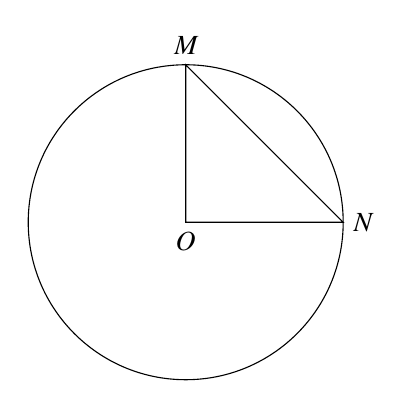
\begin{tikzpicture}
    \draw (0,0) circle (2cm);
    \draw (0,0) node[anchor=north]{$O$}
        -- (0,2) node[anchor=south]{$M$}
        -- (2,0) node[anchor=west]{$N$}
        -- cycle;
\end{tikzpicture}
\end{figure}

\solution
\begin{table}[ht]
    \begin{table}[ht]
\renewcommand\thetable{1}
\begin{tabular}{|c|c|c|}
    \hline 
    \textbf{Parameter}&\textbf{Description} &\textbf{Value}\\
    \hline 
    $r_i$ & Common ratio of G.P (a),(b),(c) & $\sqrt{2}, \sqrt{3}, \frac{1}{3}$ \\
    \hline 
    $x_i\brak{n}$ & Sequence & $x_i\brak{0}r_i^nu[n]$ \\
    \hline 
	$X_i\brak{z}$ & Transform of $x_i\brak{n}$ & $\frac{x\brak{0}}{1-rz^{-1}}$ \\
    \hline
\end{tabular}

\caption{Table of parameters}
\label{Table:1}
\end{table}

\end{table} \\
By \tabref{Table:1},
\begin{align}
    A &= \frac{1}{2}\pi \, ON \cdot OM = 50{cm}^2\\
    \because r &= ON = OM\\
    \frac{1}{2}\pi r^2 &= 50{cm}^2\\
    \implies r &= 10cm\\
    \implies A_c &= \pi r^2 = 100\pi
\end{align}

\end{document}
